% compile this on sharelatex.com
% !TEX program = pdflatex

\documentclass{scrartcl}
\usepackage[utf8]{inputenc}
\usepackage{graphicx}
\usepackage{float}

\graphicspath{ {img/} }

\title{Submission Sheet 2}
\author{Danny Heinrich \and Matthias Kasperidus \and Leonard Kleinhans}
\date{12. November 2014}



\usepackage{amsmath}

\newcommand*\colvec[2]{
        \begin{pmatrix} #1 \\ #2 \end{pmatrix}
}

\begin{document}
\maketitle

\section{Exercise 2.1: Modeling with RBF networks}
For this task we implemented a Radial Basis Function Net in R. Given a certain input of training data as well as the corresponding output one is able to train the net in such way, that a weight vector 
for given data can be obtained. Using the Gaussian basis function one can compute the differing acitvation functions in the neurons, which depend on  the euclidean norm of the difference between the input vector and
a given center. The resulting weight vector is dependent on the number of neurons as well as the value. The Gaussian basis function is defined as follows :
\begin{align*}
\phi (r) = e^{(-\frac{r^2}{\sigma^2})} 
\end{align*}
The variable r is the radius of the radial function and is defined as follows with q being the index of the neuron and x the input vector.
\begin{align*}
r = ||x-c_q||
\end{align*}

Choosing a high number of neurons relative to given inputs results in a near zero determinant. This then results in the inability of R to solve the invert of the matrix. The same goes for any given $\sigma$ . Choosing a $\sigma$ close to zero or as a multiple of the number of inputs results in a very small determinant and therefore a weight vector, which exceeds the give interval of $\ [-300,300]$.
To use the provided code load the functions into your R-Studio and call the function RBFnet with 3 arguments. For example to train a RBFN with $ q = 15$ Neurons and $\sigma = 30$ use the following syntax : 
RBFnet("path/to/function1.txt",15,30)
\begin{figure}[ht]
\begin{center}
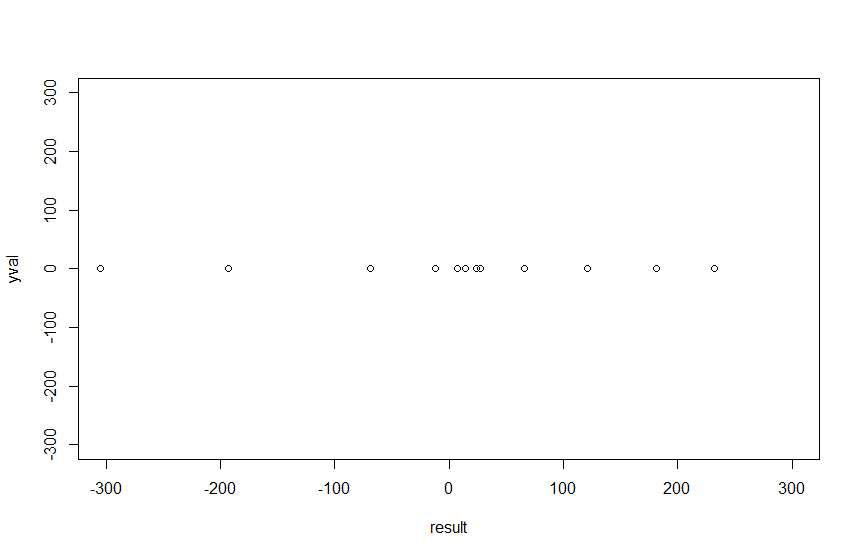
\includegraphics[scale=0.5]{RBF.png}
\end{center}
\caption{RBF Plot of 15 Neurons.}
\label{Img:RBFNetPlot}
\end{figure}

\section{Exercise 2.2: Weights for RBF}

a)
\begin{align*}
  min \left\{ || P w-y ||^2\right\} &\\
 \Leftrightarrow  \frac{\partial}{\partial w} \left( (P w-y)^T (P w-y)\right) & = 0 \\
 \Leftrightarrow  \frac{\partial}{\partial w} \left( (w^T P^T -y^T) (P w-y)\right) & = 0 \\
 \Leftrightarrow  (w^T P^T -y^T) \cdot \frac{\partial}{\partial w} \left( P w-y\right) + \frac{\partial}{\partial w} \left( w^T P^T -y^T \right) \cdot (P w-y) & = 0 \\
 \Leftrightarrow  (w^T P^T -y^T) \cdot  P + P^T \cdot (P w-y) & = 0 \\
 \Leftrightarrow  w^T P^T P - y^T P + P^T P w - P^T y & = 0  \\
 \Leftrightarrow  2 P^T P w - 2 P^T y & = 0 \\
 \Leftrightarrow  P^T P w - P^T y & = 0 \\
 \Leftrightarrow  P^T P w & = P^T y \\
 \Leftrightarrow w & = (P^T P)^{-1} P^T y
\end{align*}

b)
\begin{align*}
      min \left\{ || P w-y ||^2 + w^T D w \right\} &\\
     \Leftrightarrow  \frac{\partial}{\partial w} \left(|| P w-y ||^2 + w^T D w\right) & = 0 \\
     \Leftrightarrow  2 P^T P w - 2 P^T y + 2 D w & = 0 \\
     \Leftrightarrow  P^T P w - P^T y + D w& = 0 \\
     \Leftrightarrow w & = (P^T P + D)^{-1} P^T y
\end{align*}


\section{Exerise 2.3: SOM}
We implemented this exercise in 2_3som.R. To get a $100\times4$-Matrix one can run randomData(). To train the obtained data, run trainsom(data, iterations, rad=NULL), where iterations is the number of iterations within the SOM (update) algorithm and rad(ius) is the inital radius of the neighborhood funtion and will be passed as radius into the som funtion. \\
The resulting projetion is a color spectrum, where the input data was clustered in such way, that similar input data points (similar colors) are mapped to a similar location. This results in a continuous color spectrum. \\
Feasible values for iterations are somewhere around 4000. 

\begin{figure}[H]
    \centering
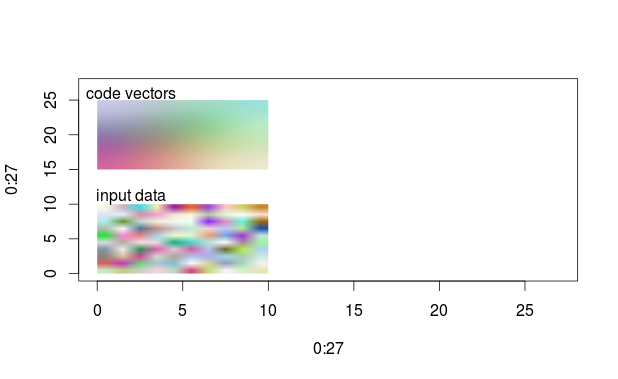
\includegraphics[width=\textwidth]{img/2_3som_sub.png}
    \caption{SOM training result}
\end{figure}


\end{document}
